%====================================================
%
% Author: Dipl.--Inf. XAVIER NOUMBISSI NOUNDOU
%
%====================================================
\documentclass[a4paper, 10pt]{report}
\NeedsTeXFormat{LaTeX2e}

%---------------------------- PACKAGE INCLUSION -------------------------------
% This group renders characters clearer and more precise

\RequirePackage[bitstream-charter,cal,expert]{mathdesign}
\RequirePackage{latexsym}

\usepackage[numbib]{tocbibind}

\usepackage{geometry}
\geometry{a4paper,
		  %showframe=true,
		  %margin=2.75em,
		  %a4paper,
		  %total={170mm,257mm},
		  top=4.3em,
		  left=3em,
		  right=3em,
		  bottom=3.39em
		  }

\usepackage{graphicx}  

\usepackage{multicol}  	  

\usepackage{caption}

\usepackage[default]{cantarell}
\usepackage{graphicx}
\usepackage{xspace}
\usepackage[parfill]{parskip} % Activate to begin paragraphs with an empty line rather than an indent
\usepackage{paralist} % very flexible & customisable lists (eg. enumerate/itemize, etc.)
\usepackage{listings} % for lstset definitions
\usepackage{url}
\usepackage{subfig} % make it possible to include more than one captioned figure/table in a single float
\usepackage{epsfig}
\usepackage{booktabs}
%\usepackage{enumitem} %funny itemize icons
\usepackage{verbatim}
\usepackage{tcolorbox}

\usepackage{pagecolor}

\usepackage{amsmath}
\newcommand{\mathbold}[1]{\text{\textbf{#1}}}

\usepackage{xcolor}
\definecolor{yerothColorOrange}{RGB}{242, 161, 0}   
\definecolor{yerothColorBlue}{RGB}{77 , 93 , 254}
\definecolor{yerothColorRed}{RGB}{254, 48 , 48}
\definecolor{yerothColorGray}{RGB}{198, 198, 198}
\definecolor{yerothColorDarkgray}{RGB}{60, 60 , 60}
\definecolor{yerothColorIndigo}{RGB}{83, 0, 125}
\definecolor{yerothColorGreen}{RGB}{2  , 160, 70}
\definecolor{forestgreen}{RGB}{2,160,70}    
\definecolor{mediumblue}{RGB}{7,43,205}    
\definecolor{firebrickred}{RGB}{178,34,34}
\definecolor{listingray}{gray}{0.9}
\definecolor{lbcolor}{rgb}{0.9,0.9,0.9}
\definecolor{darkgreen}{rgb}{0,0.35,0}
\definecolor{medgreen}{rgb}{0,0.5,0}
\definecolor{lightgreen}{rgb}{0.5,0.7,0.5}
\definecolor{pmcolour}{rgb}{0.5,0.7,0.5}
\definecolor{medgrey}{rgb}{0.6,0.6,0.6}
\definecolor{purplish}{rgb}{0.4,0,0.6}
\definecolor{brightred}{rgb}{1,0.2,0.2}

\newcommand{\diplinfn}{Dipl.--Inf.\xspace}

\newcommand{\yerothrd}{\textcolor{yerothColorGreen}
			{\textsc{\textcolor{yerothColorRed}{YEROTH}}$_{\text{r\&d}}$\xspace}}

\newcommand{\mytime}[2]{$#1$:$#2$\xspace}

\newcommand{\debianlinux}{\texttt{Debian--Linux}\xspace}

\newcommand{\windowsten}{\texttt{MS Windows $10$}\xspace}

\newcommand{\webbrowserbased}{web--browser--based\xspace}

\newcommand{\yerotherpblack}{YEROTH--ERP--$3.0$\xspace}

\newcommand{\yerotherp}{\textsc{\textcolor{yerothColorBlue}{YEROTH--ERP--$3.0$}}\xspace}

\newcommand{\saperp}{'SAP Business One'\xspace}

\newcommand{\sageerp}{'Sage Gescom i$7$'\xspace}

\newcommand{\myfullacademicname}{Dipl.--Inf. XAVIER NOUMBISSI NOUNDOU\xspace}

\usepackage{hyperref}
\hypersetup{
    colorlinks,
	pagebackref,
    citecolor=medgreen,
    linkcolor=purplish,
    breaklinks,
    pdftex,
    bookmarks,
    plainpages=false,
	pdftitle={The software--system architecture of \yerotherpblack.
			Authored by: ''\myfullacademicname''.},
    pdfauthor={\myfullacademicname}
}

%--------------------------------------------------------------------------------

%---------------------------- COMMANDS DEFINITION -------------------------------
\newcommand{\diplinf}{\emph{Dipl.-Inf.}\xspace}
\newcommand{\mycheckmark}[1]{\textcolor{#1}{$\checkmark$}\xspace}

\newcommand{\myenumitem}[1]{\emph{#1}\xspace}
\newcommand{\yerenalert}{\emph{yeren-alert}\xspace}

\newcommand{\erpsoftware}{ERP~software--system\xspace}

\newcommand{\wy}{WYSIWYG\xspace}

\newcommand{\thickclient}{thick--client\xspace}

\newcommand{\ministudio}{\texttt{miniStudio (vxWorks)}\xspace}

\newcommand{\qtdesigner}{\texttt{Qt designer}\xspace}

\newcommand{\cplusplus}{\texttt{C++}\xspace}

\newcommand{\definition}[1]{\textbf{\textcolor{yerothColorBlue}{\section{#1}}}\xspace}

\newcommand{\yerothvert}[1]{\textcolor{yerothColorGreen}{#1}\xspace}
\newcommand{\yerothrouge}[1]{\textcolor{yerothColorRed}{#1}\xspace}

\newcommand{\featuresummary}[2]{\textbf{\textcolor{#1}{\textsc{#2}}}}

%--------------------------------------------------------------------------------

\usepackage[T1]{fontenc}
\newcommand{\changefont}[3]{
\fontfamily{#1} \fontseries{#2} \fontshape{#3} \selectfont}
\changefont{cmss}{m}{n}

\renewcommand\labelenumi{\theenumi)}

\pagenumbering{arabic}

\usepackage{fancyhdr}
\pagestyle{fancy}
\renewcommand{\headrulewidth}{0pt}
\rhead{\textbf{\yerothrd}}
\lhead{The Software--System Architecture Architecture of \yerotherpblack}
\lfoot{{\small Developer: \myfullacademicname}}
\rfoot{{\small Version of --~\today~--}}
\cfoot{\thepage}

\clubpenalty = 10000
\widowpenalty = 10000
\displaywidowpenalty = 10000

\fancypagestyle{OnlyFirstPage}{%
	\lhead{}
	\rhead{}
    \lfoot{}
}

\begin{document}

\thispagestyle{OnlyFirstPage}

{\bf \Large \yerothrd} {| \sc \scriptsize the software--system architecture of \yerotherpblack}
\\ \line(1,0){540}

\vspace{2.0em}

\begin{center}
{\LARGE The Software--System Architecture of \yerotherpblack}
\end{center}

\vspace{2.0em}

\begin{center}
{\large \myfullacademicname}
\end{center}

\vspace{5.0em}

\begin{abstract}
\begin{center}
\parbox{42em}{
This document describes the architecture of our
\erpsoftware \yerotherpblack.
This document also explains the reasons for our
choice to design and build \yerotherpblack as
a \thickclient application, as opposed to
currently more popular \webbrowserbased
applications.
}
\end{center}
\end{abstract}

% TABLE OF CONTENTS
\phantomsection
%\addcontentsline{toc}{chapter}{\contentsname}
\begingroup
\tableofcontents
\endgroup

% LIST OF FIGURES
\phantomsection
%\addcontentsline{toc}{chapter}{\listfigurename}
\begingroup
\color{medgreen}
\listoffigures
\endgroup

% LIST OF TABLES
\phantomsection
%\addcontentsline{toc}{chapter}{\listtablename}
\begingroup
\color{medgreen}
\listoftables
\endgroup

\cleardoublepage

\section{Developer Biography}\label{chap:biography}
\vspace{-0.9em}

\begin{center}

\includegraphics[scale=0.32]{../../francais/images/XavierNOUNDOU-2}
\captionof{figure}{Portrait of PR. XAVIER.\label{fig:xaviernoumbis}}
\end{center}

\textbf{\myfullacademicname} is a CHRISTIAN BY FAITH,
Cameroonian, born on September~$16$ $1983$ in
DOUALA (LITTORAL region, CAMEROON).

Xavier has a \textit{''Diplom--Informatiker (Dipl.--Inf.)''}
qualification from the \textbf{\unibremen, Bremen, Bremen, GERMANY} (May~$25$, $2007$).

Xavier is a \textit{PH.D. in Software Engineering}
(software construction, and testing) since November~$18$,~$2020$
because of his academic research, and professional engineering
contributions as follows:


\begin{enumerate}
%	\itemsep -0.7em
	\item 'Context-Sensitive Staged Static Taint Analysis
			For C using LLVM'
		\begin{enumerate}[1.]
			\itemsep -0.7em
			\item source code: \\
			\url{http://github.com/xnoumbissinoundou/yeroth-saint}
			\item full text (published on July~$1^\text{st}$, $2015$): \url{http://archive.org/details/saint_201507}.
		\end{enumerate}		 

	\item 'YEROTH-ERP-3.0':
			\begin{enumerate}[1.]
			\itemsep -0.7em
			\item source code: \\
			\url{http://github.com/xnoumbissinoundou/yeroth-erp-3.0}
			\item full text (ongoing publication): \url{http://archive.org/details/yeroth-erp-3-0-info-english}.
		\end{enumerate}	
\end{enumerate}


\chapter{Introduction}\label{chap:introduction}

\yeren est un syst\`eme logiciel de gestion des
stocks et de gestion des ventes. Il permet
d'ex\'ecuter des mouvements de stocks, et de
vendre des articles en stocks.

Une entreprise doit poss\'eder au minimum d'un stock
d'articles, d'un d\'ep\^ot ou d'une boutique pour utiliser
\yeren de fa\c{c}on efficace.\\

\begin{figure}[!htpb]
	\centering
	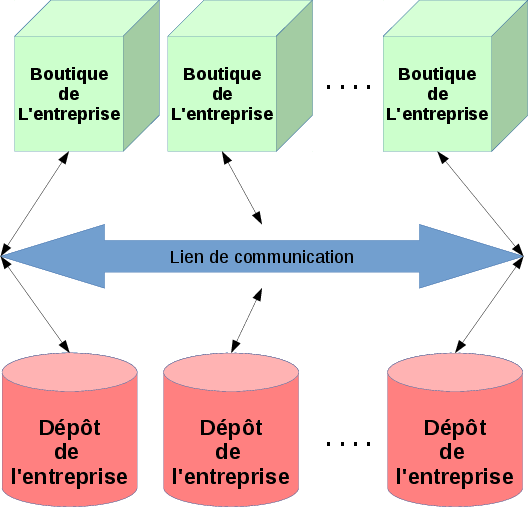
\includegraphics[scale=0.63]{images/architecture-enterprise-yeren.png}
	\caption{Un mod\`ele d'architecture d'une entreprise}\label{fig:architecture-enterprise-yeren}
\end{figure}

La figure~\ref{fig:architecture-enterprise-yeren} illustre
un mod\`ele g\'en\'erique d'entreprise o\`u les d\'ep\^ots
et les boutiques de l'entreprise sont en communication.

Les activit\'es principales de l'entreprise sont les suivantes:
\begin{enumerate}[1)]
	\item \emphbf{les sorties de stocks:} sortie d'articles
		d'une unit\'e (boutique ou d\'ep\^ot) pour r\'eception par un client
	\item \emphbf{les transferts de stocks:} mouvement d'articles
		d'une unit\'e vers une autre unit\'e
	\item \emphbf{les ventes d'articles:} un client ach\`ete
		des articles qui lui sont ensuite remis.\\
\end{enumerate}

\yeren permet d'accomplir les t\^aches de gestion
des stocks et de gestion des ventes suivantes:
\begin{enumerate}[1)]
	\item \myenumitem{cr\'eer des alertes sur des p\'eriodes de temps}	
	\item \myenumitem{cr\'eer des alertes sur des quantit\'e en stocks}	
	\item \myenumitem{entrer un stock}
	\item \myenumitem{lister les stocks}
	\item \myenumitem{modifier un stock}
	\item \myenumitem{supprimer un stock}	
	\item \myenumitem{rechercher des articles ou des stocks}
	\item \myenumitem{transf\'erer des articles ou des stocks}	
	\item \myenumitem{vendre des articles}	
	\item \myenumitem{visualiser les \'etats de transactions d'articles
		(sorties ou transferts de stocks)}
	\item \myenumitem{acc\'eder aux tableaux de bords}
	\item \myenumitem{visualiser les \'etats de ventes d'articles}.\\
\end{enumerate}

\newpage

\section{Acc\`es au manuel de l'utilisateur}

La figure~\ref{fig:fenetre-principale-utilisateur-non-enregistre}
illustre la fen\^etre d'accueil de \yeren sans aucun utilisateur
enregistr\'e.\\

\begin{figure}[!htbp]
\centering
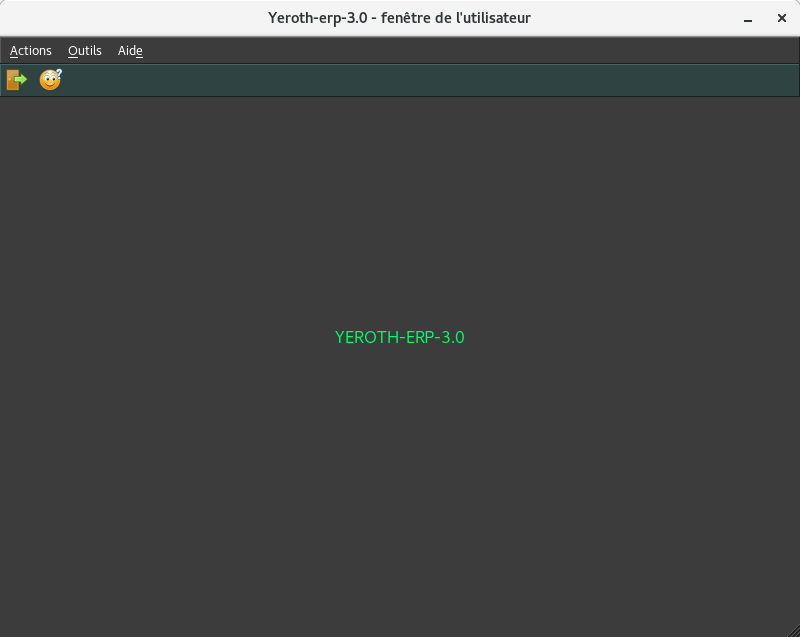
\includegraphics[scale=0.63]{images/yeren-fenetre-principale.png}
\caption{La fen\^etre d'acceuil sans aucun utilisateur enregistr\'e.}
\label{fig:fenetre-principale-utilisateur-non-enregistre}
\end{figure}

Il est requis qu'un utilisateur soit enregistr\'e
dans \yeren afin d'avoir acc\`es au manuel de l'utilisateur.

L'utilisateur de \yeren doit accomplir les op\'erations
suivantes afin d'avoir acc\`es au manuel de l'utilisateur:
\begin{enumerate}[1)]
	\item \`a partir de la fen\^etre d'accueil
		(voir figure~\ref{fig:fenetre-principale-utilisateur-non-enregistre}),
		cliquez sur le menu d\'eroulant '\textbf{Aide}'
	\item ensuite cliquez sur le lien '\textbf{Manuel de l'utilisateur (PDF)}'.
\end{enumerate}

\section{Structure de ce manuel de l'utilisateur}
Ce manuel de  l'utilisateur de \yeren est structur\'e
comme suit:

\begin{itemize}[\mycheckmark{purplish}]
	\item le chapitre~\ref{chap:utilisateurs} d\'ecrit
	les utilisateurs de \yeren et leurs \roles. 
	     
	\item le chapitre~\ref{chap:gestion-stocks} explicite
	les fonctionalit\'es de gestion des stocks

	\item le chapitre~\ref{chap:gestion-des-achats} parle
	de la gestion des achats
	
	\item le chapitre~\ref{chap:systeme-dalertes}
	pr\'esente le syst\`eme d'alertes sur les stocks
	
	\item le chapitre~\ref{chap:vendre} d\'ecrit comment
	conclure des ventes d'articles
	
	\item le chapitre~\ref{chap:sortir-articles} d\'ecrit
	comment proc\'eder \`a des sorties et transferts de stocks
	
	\item le chapitre~\ref{chap:vente} explicite comment
	rechercher et imprimer les \'etats de ventes d'articles
	
	\item le chapitre~\ref{chap:etats-des-sorties} explicite
	comment rechercher et imprimer les \'etats de sorties ou
	transferts d'articles
	
	\item le chapitre~\ref{chap:tableaux-de-bord} discute
	de la recherche et de la g\'en\'eration des rapports
	commerciaux de l'entreprise
	
	\item le chapitre~\ref{chap:informations-generales}
	explique comment avoir acc\`es aux d\'etails de
	l'utilisateur enregistr\'e, aux informations commerciales
	de l'entreprise, et enfin \`a la version de \yeren que
	l'on utilise
	
	\item le chapitre~\ref{chap:administration-logiciel}
	traite de l'administration du logiciel

	\item le chapitre~\ref{chap:problemes-connues}
	discute des probl\`emes connues de \yeren
	
	\item enfin, le chapitre~\ref{chap:conclusion} conclut
	ce manuel d'utilisation.
\end{itemize}



\chapter{Thick--Client VS Web--Browser--based
	Software--System Architecture}


\begin{table*}[!htbp]
\centering
\resizebox{\textwidth}{!}{%to fit the table within the text width
\begin{tabular}{cccc} 

\multicolumn{1}{c}{}										&
Thick--client application \mycheckmark{yerothColorBlue}	& 
Web--browser--based application								\\ \hline

business code								&
		\yerothrouge{all computers}			&						
		\yerothvert{application server}		\\ \hline
		
co--related software--systems		&
		\yerothvert{$1$ (DBMS)}		&						
		\yerothrouge{at least $3$ (DBMS, web~/~application server)}	\\ \hline
				
user interface											&
		\yerothvert{all computers (\thickclient gui)}	&						
		\yerothvert{all computers (web--browser)}		\\ \hline		
		
number of logical layers									&
		\yerothvert{$2$ (client and data)}					&						
		\yerothrouge{$4$ (client, presentation, logic, and data)}\\ \hline
				
rapid prototyping (\wy tools)		&
		\yerothvert{yes}			&						
		\yerothrouge{very limited}	\\ \hline				
				
software security vulnerability										&
		\yerothvert{low ($1$ programming language)}		&					
		\yerothrouge{high (\emph{several} programming languages)}	\\ 
\end{tabular}}
\caption{Thick--client application VS Web--browser--based application.\\}
\label{tab:thickclient-application-againts-webbrowserbased-application}
\end{table*}

\begin{center}

\includegraphics[scale=0.52]{images/yeroth-thickclient-application-two-tier-architecture.png}
\captionof{figure}{$2$--layers logical 
architecture of \thickclient software--system 
(copied from \cite{securityboulevarddotcom:2020}).}
\label{fig:yeroth-thickclient-application-two-tier-architecture}
\end{center}

Figure~\ref{fig:yeroth-thickclient-application-two-tier-architecture}
illustrates an example of a \thickclient
software--system with a $2$--layers
logical architecture.

\begin{center}
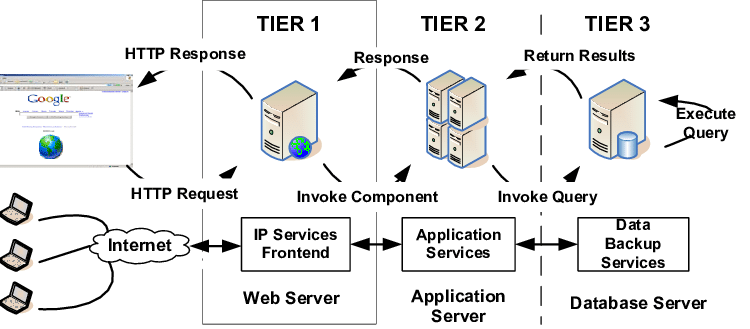
\includegraphics[scale=0.39]{images/yeroth-three-tier-architecture.png}
\captionof{figure}{$4$--layers logical architecture
of \webbrowserbased software--system
(copied from \cite{trevor:2006}).}
\label{fig:yeroth-three-tier-architecture}
\end{center}

Figure~\ref{fig:yeroth-three-tier-architecture}
illustrates an example of a \webbrowserbased
software--system with a $3$--layers
logical architecture.

Table~\ref{tab:thickclient-application-againts-webbrowserbased-application}
compares \thickclient software--systems against
\webbrowserbased software--systems.

\chapter{The Thick--Client Software--System Architecture of \yerotherpblack}


\section{Business and user interface code deployment}

Table~\ref{tab:thickclient-application-againts-webbrowserbased-application}
depicts the issue of business and user
interface code deployment on all computers
participating in the functioning of \yerotherpblack,
as a software--system for a user.

We tackle the problem of automatic deployment of
business and user interface code on all user
computers by using the '\texttt{apt upgrade}'
software--system on '\debianlinux'.

\section{Co--related software--systems}


\section{User interface}


\section{Number of logical layers}


\section{Software security vulnerabilities}

\subsection{Vulnerability detection}

\subsection{Vulnerability prevention}

\subsection{Vulnerability protection}

\chapter{Related Software--System Architectures}

\chapter{Conclusion}

\yerotherpblack has a \thickclient
software--system architecture because we
found \thickclient software--system
architectures simpler than \webbrowserbased
software--system architectures.

A \webbrowserbased software--system
architecture has more drawbacks as
follows:

\begin{enumerate}[1)]
	\item it requires at least $3$ co--related 
		software--systems are required 
		(e.g.: DBMS, web server, application server.)
		to fully operate.
		
	\item A \webbrowserbased software--system
		requires at least $4$ layers within
		its logical system architecture
		(e.g.: client, presentation, logic, and data).

	\item A \webbrowserbased software--system
		potentially possesses more software
		security vulnerabilities because its
		implementation requires of the use of
		at least $2$ different programming 
		languages, and frameworks in combination.
\end{enumerate}

Table~\ref{tab:thickclient-application-againts-webbrowserbased-application}
demonstrates \thickclient software--system architecture
is better than \webbrowserbased software--systems.

\cleardoublepage
\bibliographystyle{alpha}
\bibliography{bibliography}

\cleardoublepage
\phantomsection
\addcontentsline{toc}{chapter}{\textsc{Appendix}}
\appendix






\end{document}

